%!TEX root = ../thesis.tex
%*******************************************************************************
%****************************** Second Chapter *********************************
%*******************************************************************************

\chapter{Systematic Uncertainties}
\label{sec:syst_uncert}

The precision of the measurement of the \ttbar cross section is typically dominated by systematic uncertainties,
even when only a comparetively small amount of data is used \cite{Khachatryan:2015uqb}. In this analysis systematic uncertainties are treated as nuisance parameters in a
template fit. This allows to reduce their impact, but also makes the exact treatment of the different sources of systematic variations important. 

In this chapter the systematic uncertainties are described in detail starting with the uncertainties based on experimental effects in Section \ref{sec:exp_uncert}.
The uncertainties based on theoretical assumptions are discussed in Section \ref{sec:theo_uncert}. If necessary the treatment of the systematics as nuisance
parameter and especially the prior that is chosen to model the behaviour of the respective nuisance parameter is discussed as well.

Broadly speaking there are two main effects of the systematic uncertainties on the templates: They can affect the normalization of the templates, the shape or both.
When looking in detail most uncertainties do affect both the shape and the normalization, but some clearly affect one more than the other.
At the same time the uncertainty can affect different categories of events differently then others or affect all events similarly.
An uncertainty on the normalization of all templates is in general harder to constrain than an uncertainty affecting the shape of the templates as the normalization of the
\ttbar template is directly tied to the cross section which is the parameter of interest. This applies especially to uncertainties applying to all events in the same way.


\section{Experimental Uncertainties}
\label{sec:exp_uncert}

\subsection{Uncertainties Related to Leptons}

The identification and reconstruction of the leptons have different efficiencies in data and simulation as described in Section \todo{cite section}.
The simulation is rescaled to model the efficiencies in data, but the efficiency measurements themselves have an uncertainty that needs to be propagated to the final measurement by varying the scale factor for the electrons or muons within its uncertainty resulting in a two sided variation.
The efficiency itself is usually measured with the Tag and Probe method, which allows to measure the efficiency independently in data and simulation as described in Section \ref{sec:TriggerTPMethod}.

For the electrons the uncertainty on the efficiency measurement is the sum of single sources taking into account alternative models for both the background contribution
and the shape of the Z boson mass peak.
The uncertainty due to the selection of the tag is evaluated by changing the tag selection in both data and MC.
These contributions are considered to be uncorrelated and added up in quadrature. 
Since the uncertainties vary based on the kinematics of the electron the electron effiency uncertainty also has a small shape effect on the templates for signal and background, but the larger effect
is on the normalization to the order of $\sim 0.5 \; \% - 2\; \%$ in the bulk of the phase space.

In contrast the muon efficiency uncertainty is estimated as an envelope of multiple effects. These include the binning and range that is used to model the Z boson mass peak as well as the variation of the assumed signal shape. As for the uncertainty on the electrons it also includes a change in the tag selection.
The total uncertainty is $1.25 \; \%$ independent of the muon kinematics, resulting in a pure normalization uncertainty.

The measured energy of the leptons needs to be scaled to account to correct the reconstruction for possible bias. In simulation the energy also needs to be smeared so the energy resolution in simulation is representative of the resoltion in data.
For both electrons and muons the corrections on simulation are varied to model the uncertainty.

For the electrons this uncertainty combines the effects of training these corrections for electrons or photons, the choice of cuts used in the training and the choice of the simulated sample that is used in the training. It also includes an uncertainty on the method itself evaluated with a closure test and a correction for a possible
dependance of the original energy of the electron.
The uncertainty on the electron energy scale and smearing are then treated as separate nuisance parameters.

For the muons the uncertainty includes amongst other contributions changing the mass range of the Z peak as well as a staistical component. The maximum deviations of each contribution are then added in quadrature to obtain the total systematic correction.

Since the measurement mainly relies on templates of jet related observables the uncertainties on the lepton energies has an effect on the number of events when an event can fail the selection
due to a different lepton energy, otherwise the impact of these uncertainties should be comparatively small.

The systematic uncertainty on the trigger efficiency measurement is described in Section \ref{sec:TrigSF}. This uncertainty is applied by varying the respective correction scale factors
and its explicitely correlated among the three lepton decay channels. Since it only weakly depends on the lepton kinematics it mainly has a normalization effect on the templates used in the fit.

\subsection{Uncertainties Related to Jets}

As described in Section \todo{Link} the templates used for the cross section measurement are based on jet related observables.
Uncertainties related to jets consequently tend to directly affect the templates. The total number of events however does only weakly depend on the properties of the jets
since there is no specific requirements on jets for events in the \emu channel.

The uncertainty on the correction of the jet energy as described in Section \todo{Link to reco chapter} is split up into 19 different sources depending on the $\pt$ and $\eta$ of the jets.
These different sources are treated as separate uncorrelated nuisance parameters.
Similar to the nominal correction the uncertainty is applied by rescaling the energy of each jet in simulation.
These sources include a comparison between the differences in the behaviour of jet fragmentation and final state radiation between Pythia6 and Herwig++ \todo{check spelling + cite}.
They also include uncertainties due to the flavor of the jet again coming from a comparison of Pythia6 and Herwig++.
Different methods to evaluate the correction of the jets themselves are compared and their difference is used as another uncertainty.
Other sources of uncertainty are the variation of the response to a single particle in both the hadronic and electromagnetic calorimeter.
The uncertainty due to the resolution of the jets is split into different regions depending on $\eta$.
The uncertainty on the estimation of pile-up is taken into account by both applying the uncertainty on the pile-up correction in simulation and comparing simulation with and without added pile-up.
Finally the depence on the changing conditions during data taking is taken into account by comparing corrections limited to a single run period with the total average.

Jets in simulation also need to be corrected to match the resolution of the jet energy in data \todo{Link}. Similar to the correction itself the uncertainty depends on the $\eta$ of the jet and on
the $\pt$ of the generated jet (before detector reconstruction). 
The uncertainty on the correction is applied to each jet separately by repeating the resolution correction with a changed scale factor. In general the impact of this uncertainty is lower than the impact 
of the uncertainty on the jet energy scale corrections.

The efficiency that a jet originating from a b quark is b-tagged is measured intrinsically together with the \ttbar cross section as explained in Section \todo{Link}. The systematic uncertainty is taken from a dedicated and unrelated measurement of the b-tag efficiency \todo{cite} using di-jet events. It is applied by reweighting simulated events according to this uncertainty. The uncertainty generally depends on $\pt$ and $\eta$ of the jet.
It takes various sources into account like the uncertainty on the simulation of B meson fragmentation, gluon splitting and further meson branching fractions.
It also considers experimental uncertainties like the impact of the jet energy scale. The uncertainty introduced through pile-up is evaluated by propagating the uncertainty
on the pile-up determination to the b-tagging efficiency measurement.
The uncertainty on the probability that a jet originating from a light quark could be b-tagged is treated in a similar way.
The effect of this uncertainty is well visible in the multiplicity of b-tagged jets in each event shown in Figure \ref{fig:control_var_BTAGH}, especially in the ratio between the data and predicition.
It also shows that the variation on the predicted number of events is larger than the statistical uncertainty on the amount of measured events, showing the potential to constrain this variation in the
template fit.

\begin{figure}[htbp!]
  \begin{center}
      \resizebox{0.32 \textwidth}{!}{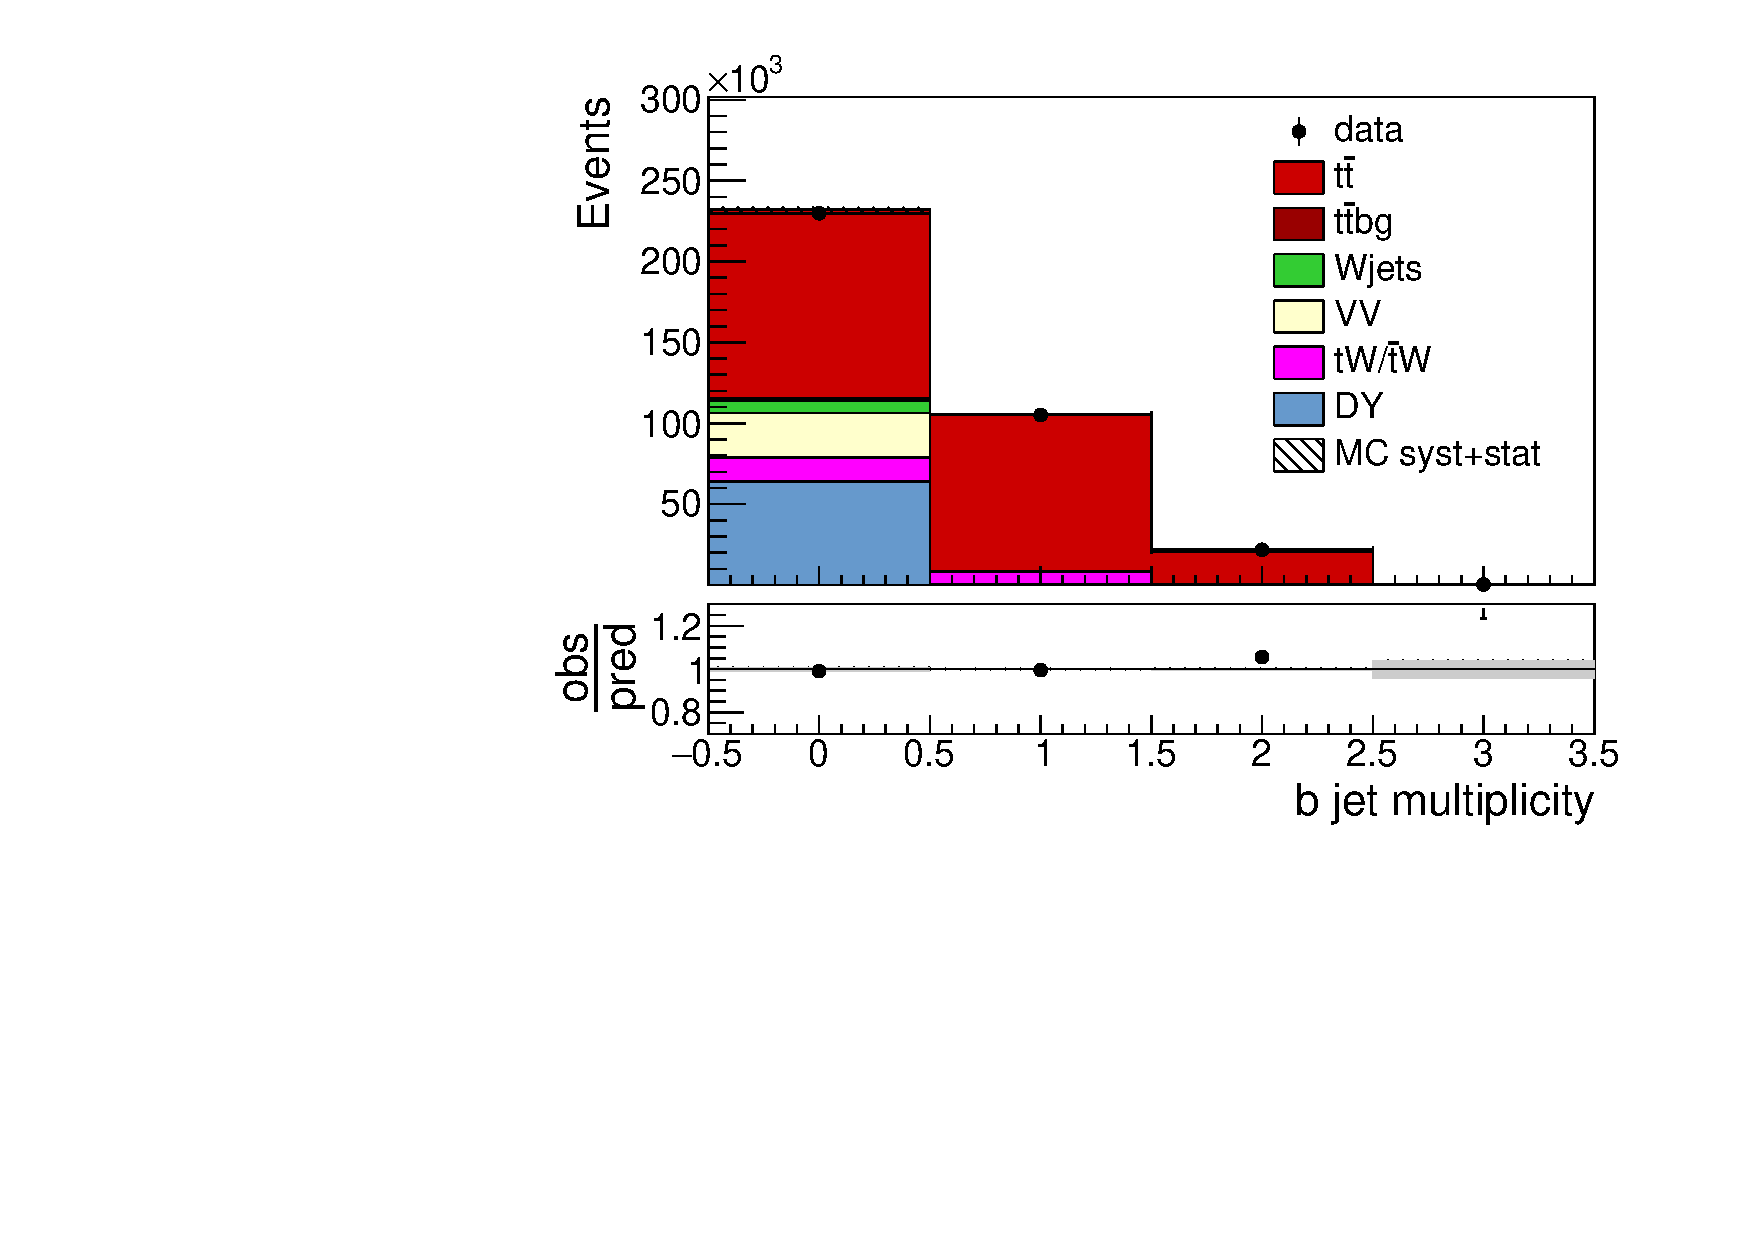
\includegraphics{SystematicUncerts/Figures/variationPlots/controlPlots/BTAGH/selected_b-jet_multi_step_8_BTAGH_down.pdf}}
    \resizebox{0.32 \textwidth}{!}{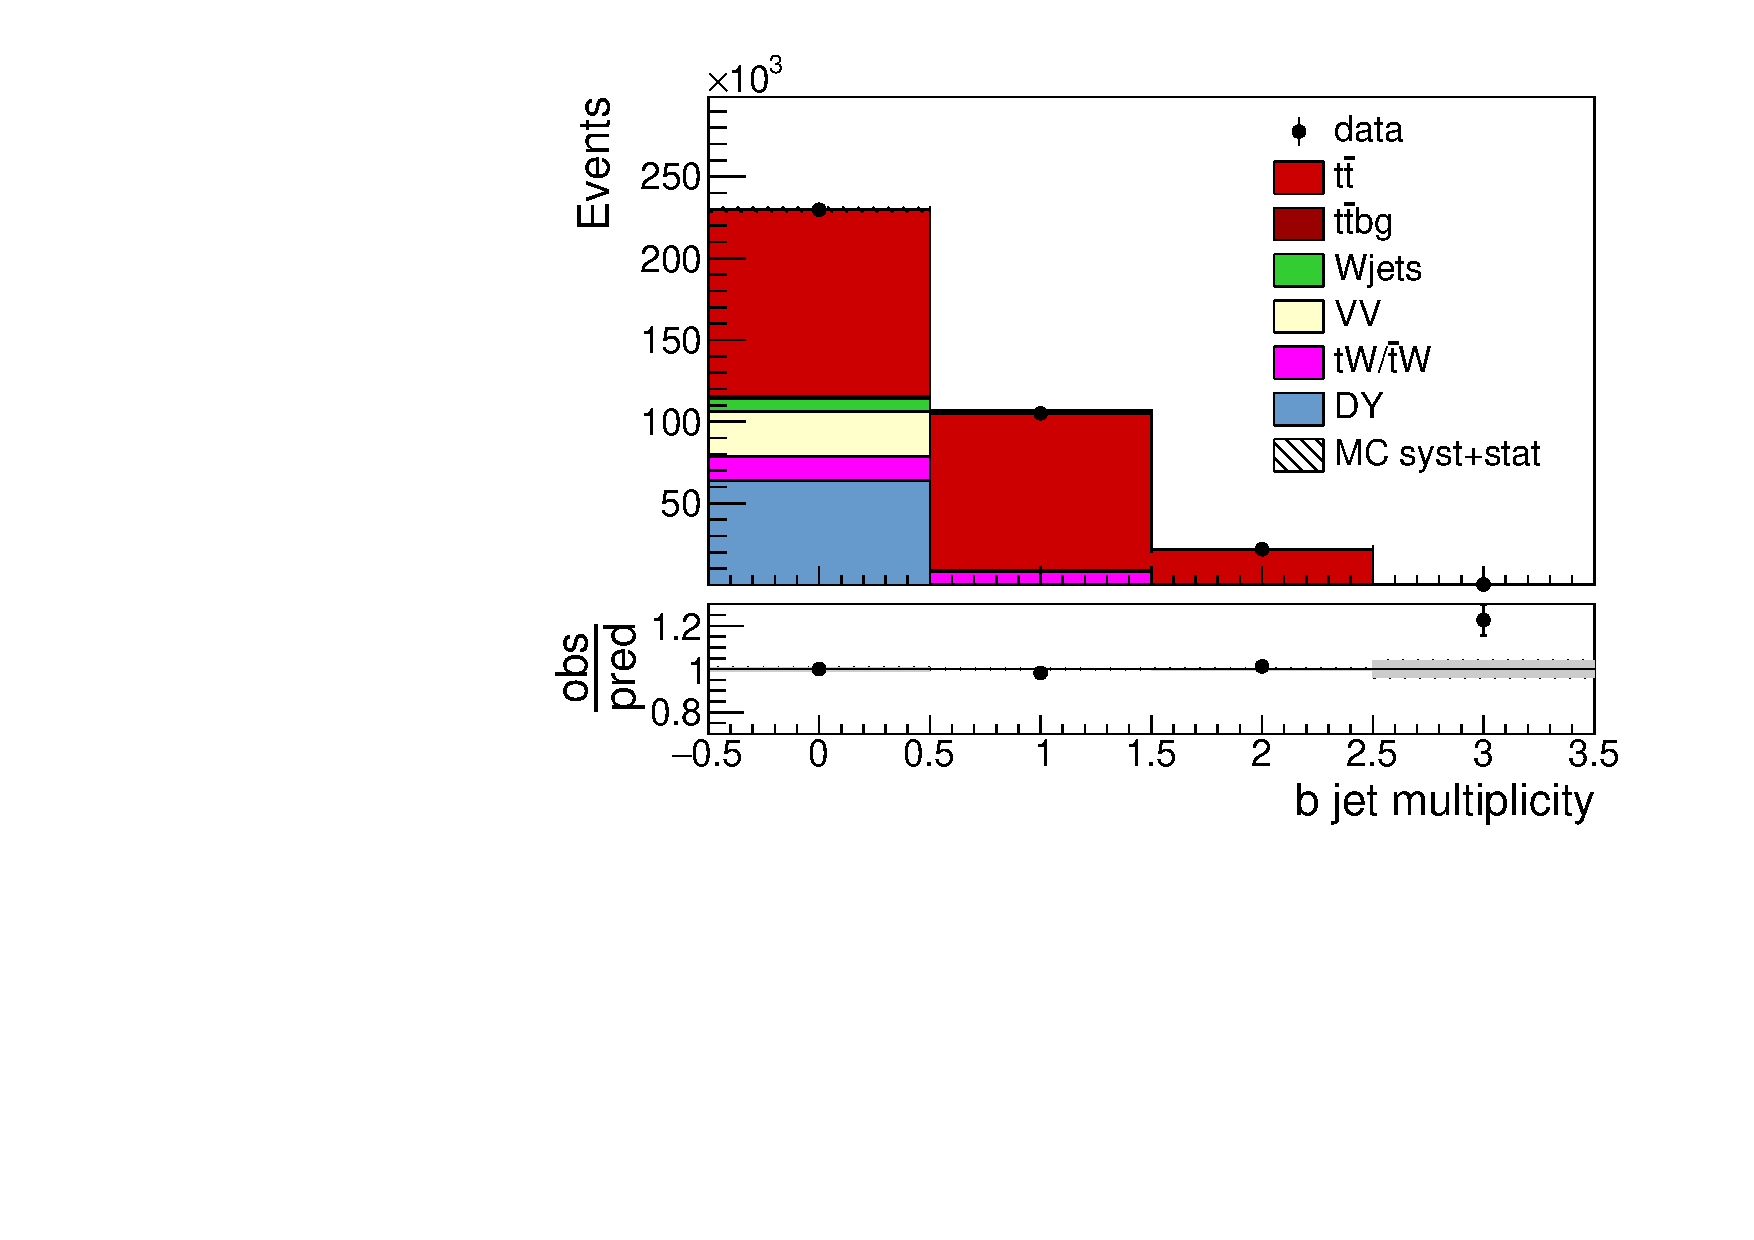
\includegraphics{SystematicUncerts/Figures/variationPlots/controlPlots/BTAGH/selected_b-jet_multi_step_8_nominal.pdf}}
    \resizebox{0.32 \textwidth}{!}{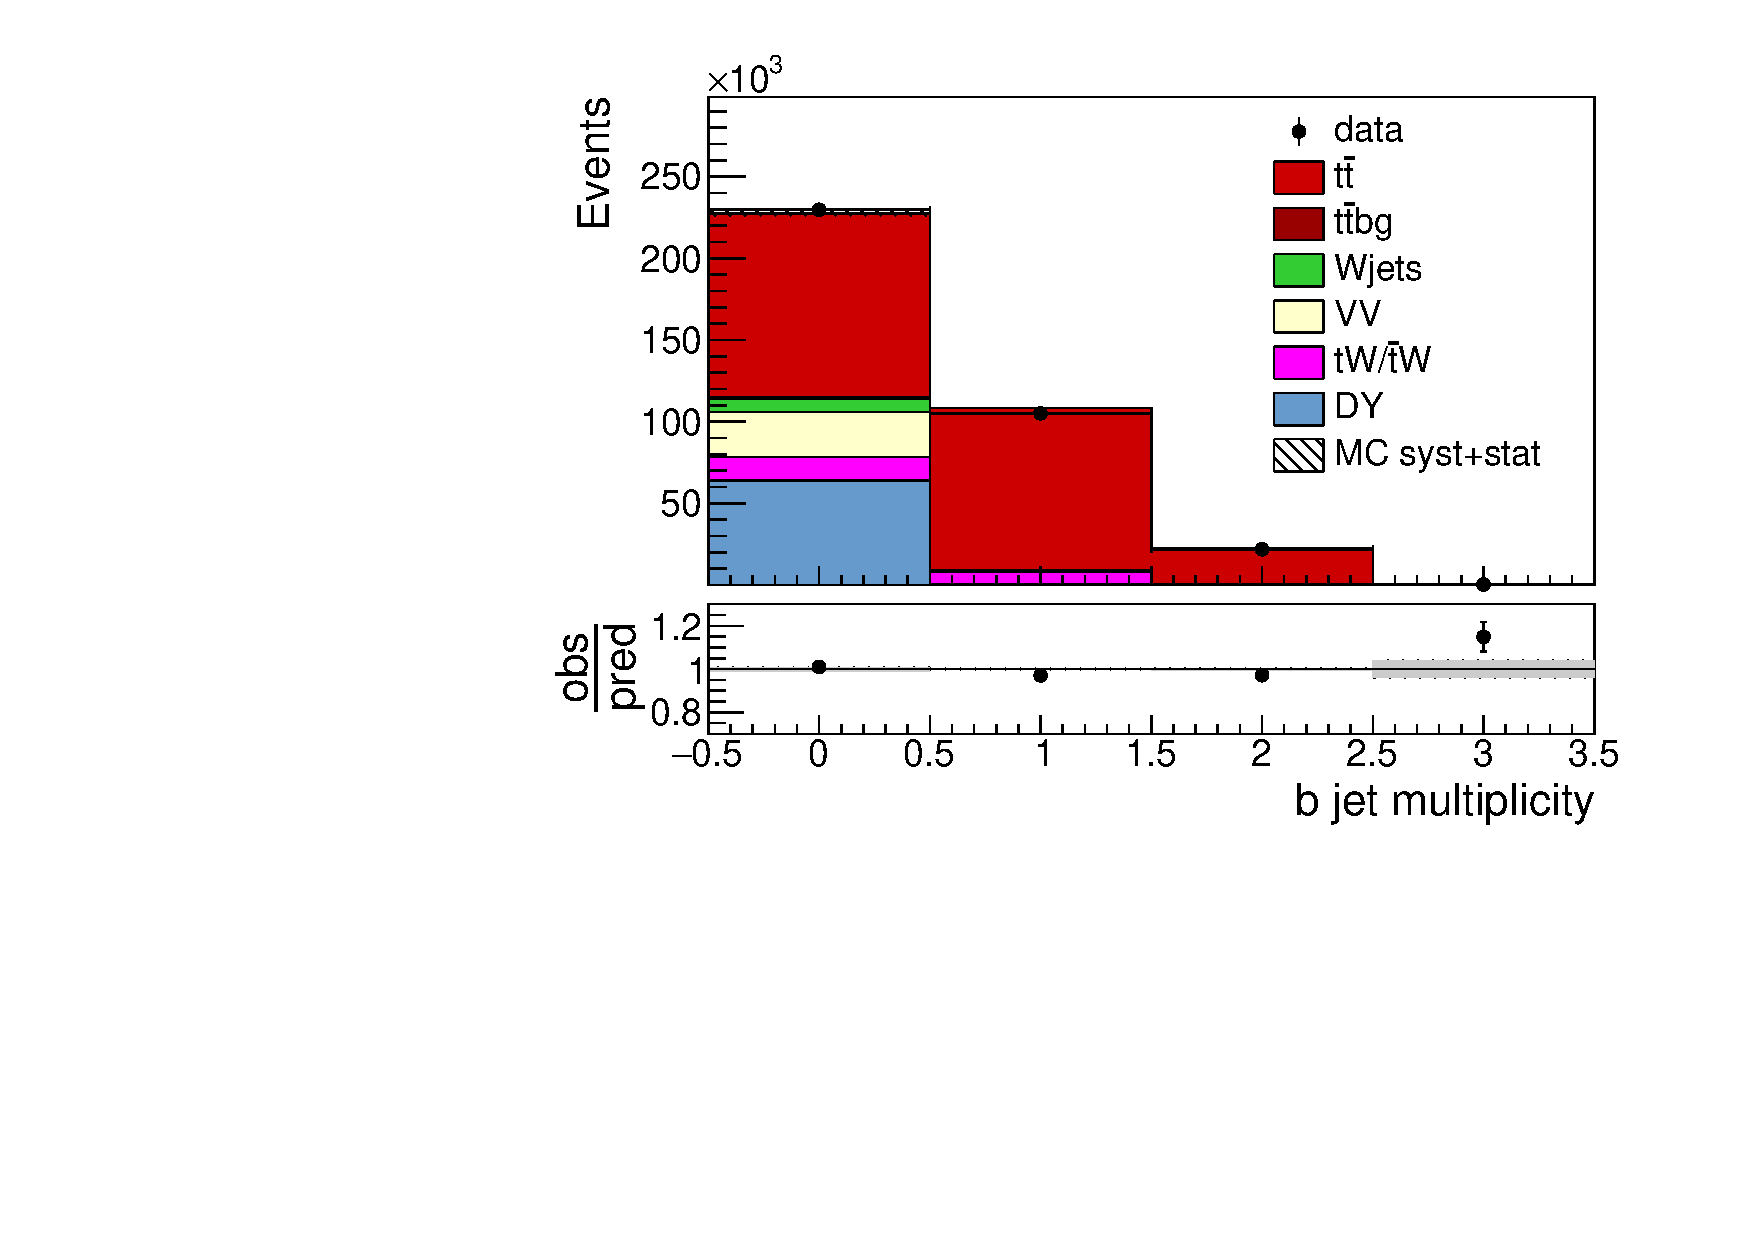
\includegraphics{SystematicUncerts/Figures/variationPlots/controlPlots/BTAGH/selected_b-jet_multi_step_8_BTAGH_up.pdf}}

\caption{Multiplicity of b-tagged jets in the \emu channel for the two systematic variations (left,right) and the nominal (middle) scale factors for the b-tagging efficiency.
The hatched bands correspond to the statistical uncertainty on the sum of the predicted yields. 
        The ratios of the event yield in data to the sum of the predicted yields are
        shown at the bottom of each plot. Here, the solid gray band
        represents the contribution of the statistical uncertainty.
  \label{fig:control_var_BTAGH}}
  \end{center}
\end{figure}


\subsection{Further Experimental Uncertainties}

The estimation of pile-up in simulation is corrected according to the assumed pile-up contribution in data. This correction is based on the total inelastic proton-proton cross section.
A weight is applied to events in simulation depending on the number of primary vertizes. To estimate the systematic uncertainty of this correction the total proton-proton cross section is changed
by $4.6 \; \%$ and new correction factors are estimated based on the changed value.
The impact of these variations is shown in the distribution of the number of primary vertices per event as shown in Figure \ref{fig:control_var_PU}.
A mismatch between measured data and simulated events is visible in the nominal distribution, but as shown in the left figure the systematic variations cover this divergence.
This can lead to a fit result for the specific nuisance parameter tied to the systematic variation being different from one.

\begin{figure}[htbp!]
  \begin{center}
    \resizebox{0.32 \textwidth}{!}{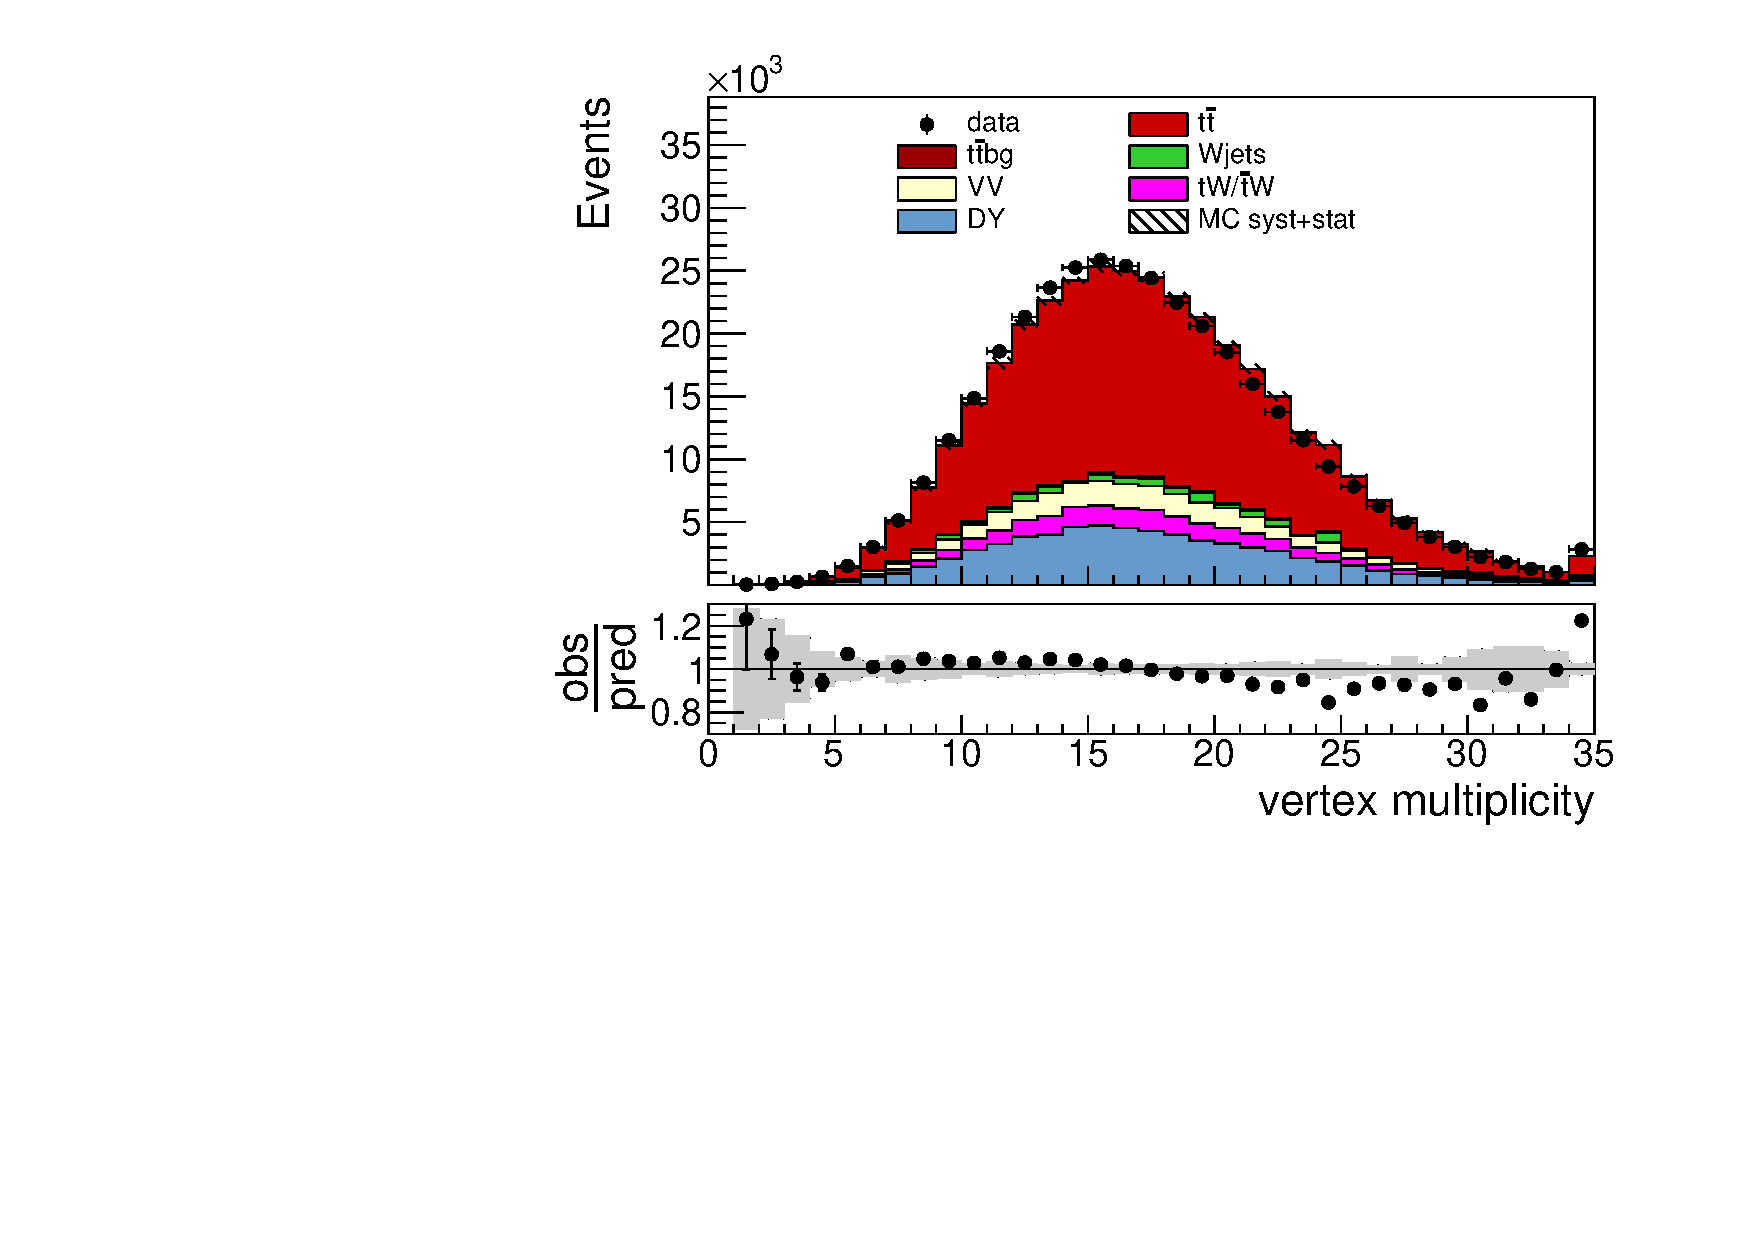
\includegraphics{SystematicUncerts/Figures/variationPlots/controlPlots/PU/vertex_multiplicity_step_8_PU_down.pdf}}
    \resizebox{0.32 \textwidth}{!}{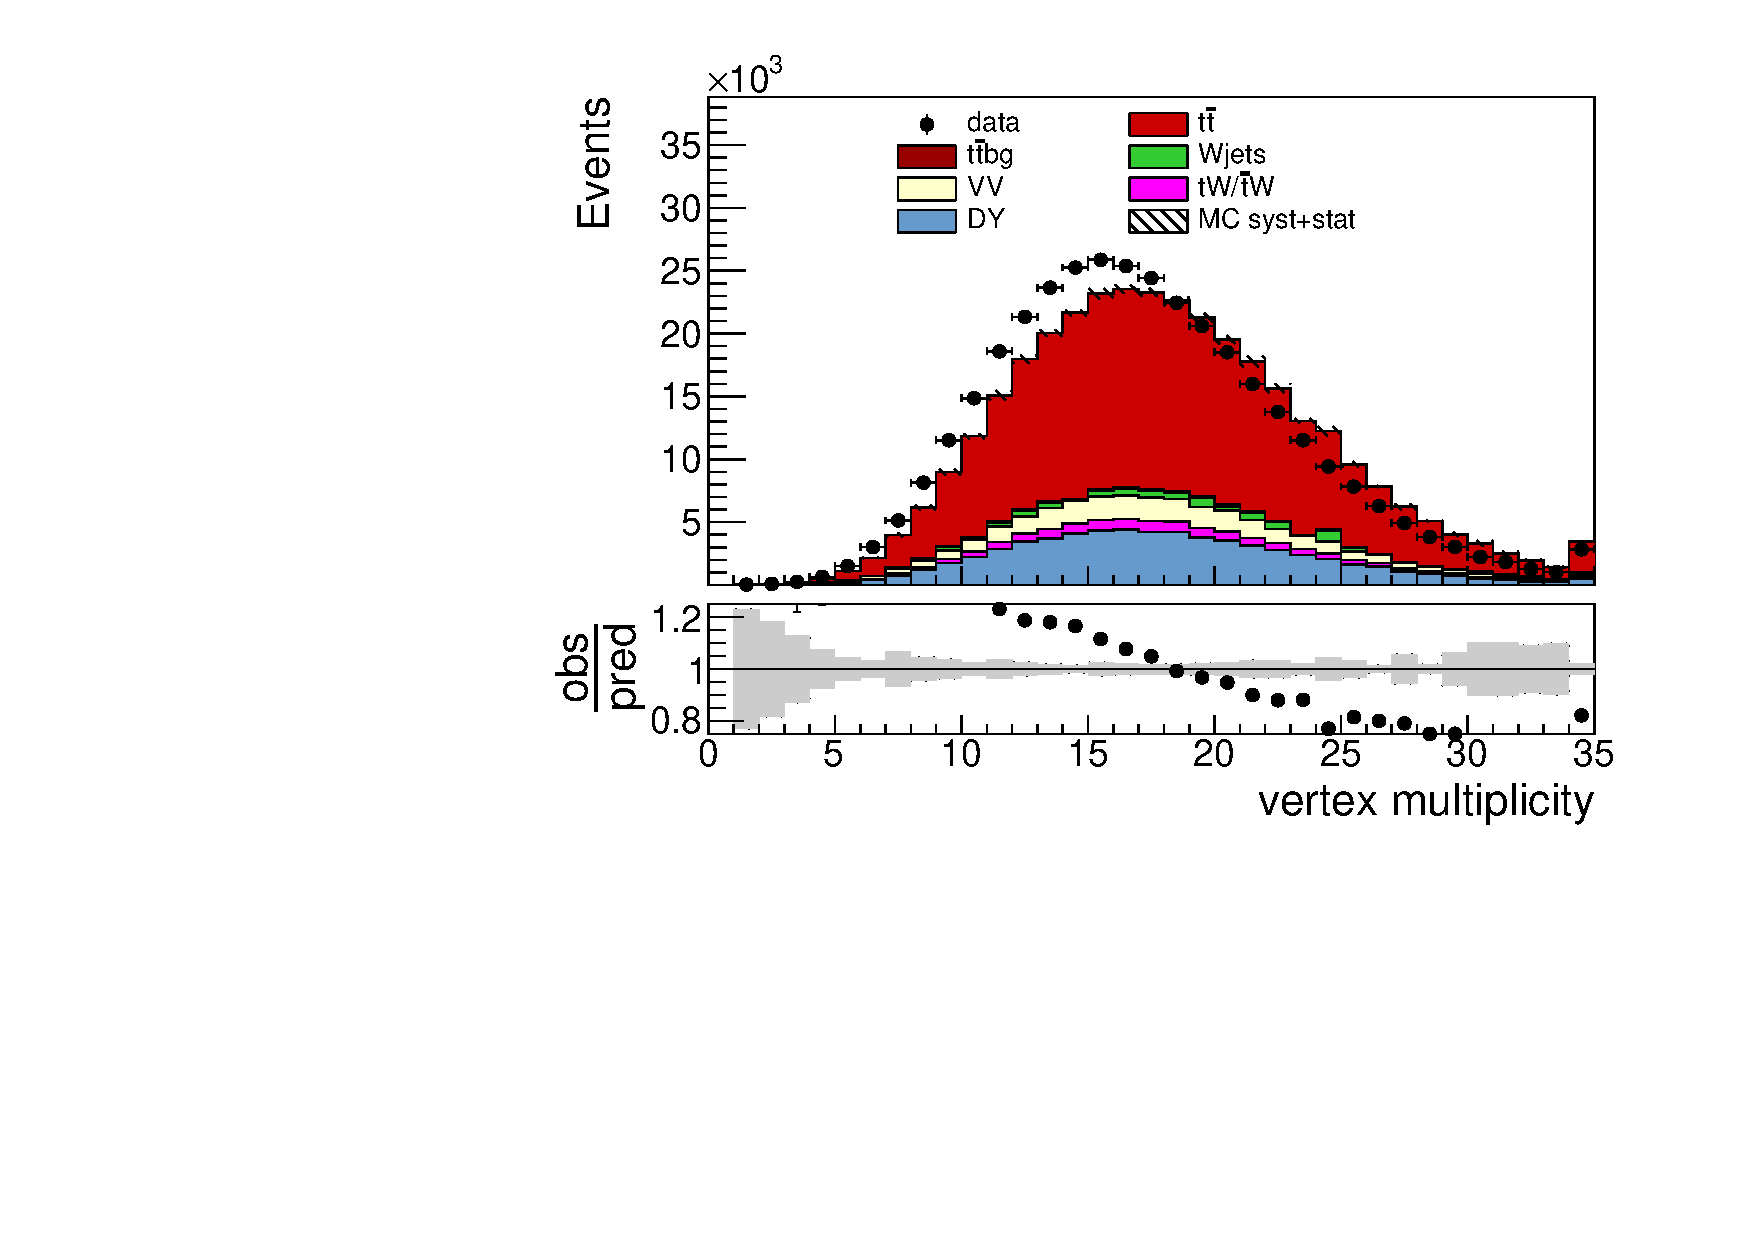
\includegraphics{SystematicUncerts/Figures/variationPlots/controlPlots/PU/vertex_multiplicity_step_8_nominal.pdf}}
    \resizebox{0.32 \textwidth}{!}{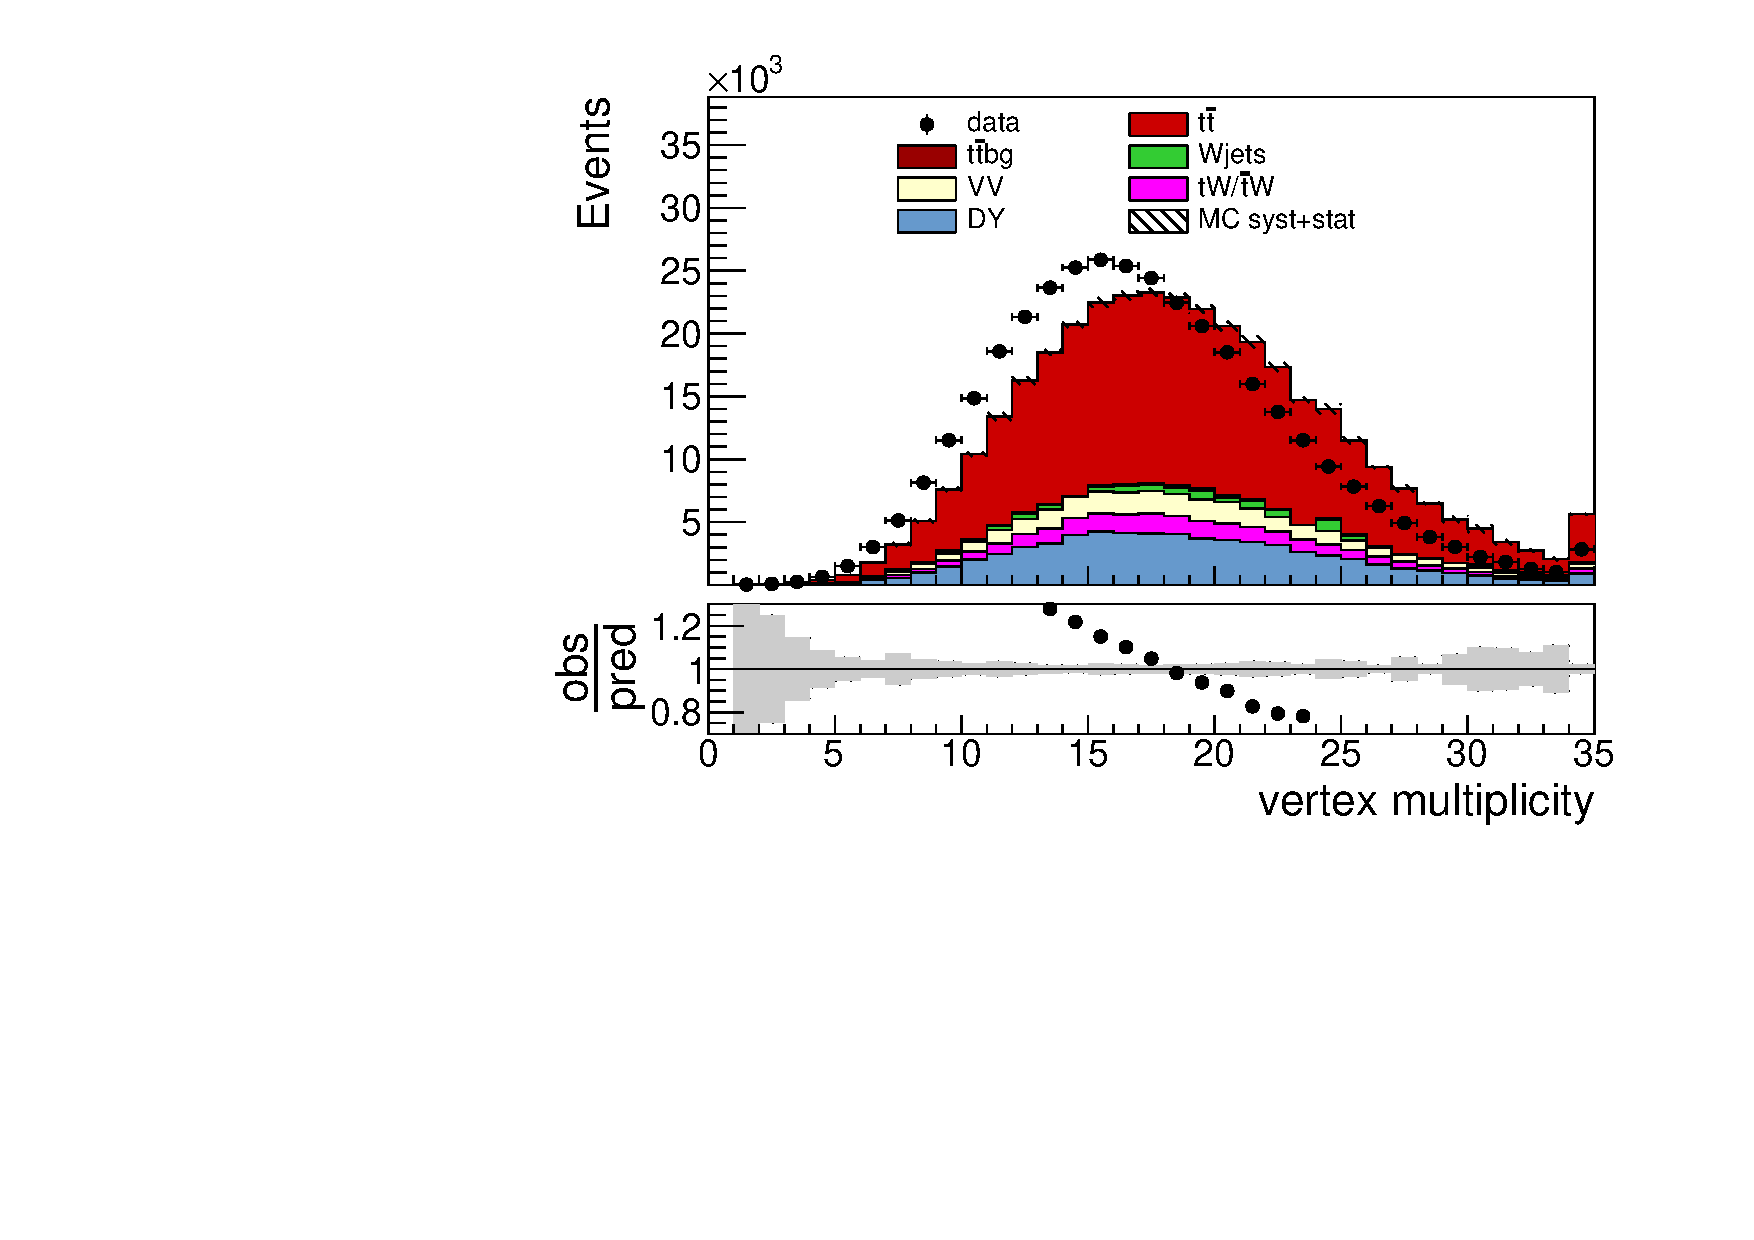
\includegraphics{SystematicUncerts/Figures/variationPlots/controlPlots/PU/vertex_multiplicity_step_8_PU_up.pdf}}
\caption{The number of primary vertices per event in the \emu channel for the two systematic variations (left,right) and the nominal (middle)  PU re-weighting.
The hatched bands correspond to the statistical uncertainty on the sum of the predicted yields. 
        The ratios of the event yield in data to the sum of the predicted yields are
        shown at the bottom of each plot. Here, the solid gray band
        represents the contribution of the statistical uncertainty.
  \label{fig:control_var_PU}}
  \end{center}
\end{figure}


The luminosity is determined by extrapolating the result of a measurement \todo{cite} of the luminosity using special proton beam conditions to the full data taking period.
The uncertainty on the luminosity is determined in a dedicated analysis by both taking into account the uncertainty on the initial measurement itself as welll as uncertainties
introduced in the extrapolation, mainly through changes in detector or beam conditions.
This systematic uncertainty is not included as a nuisance parameter in the fit. It is externalised by directly applying it on the final results of the cross section measurement.

\section{Theoretical Uncertainties}
\label{sec:theo_uncert}

The simulation of the \ttbar signal has a strong impact on the measurement of the \ttbar cross section.
Since it is based on multiple theoretical assumptions it is important to assess the uncertainty introduced through reasonable variations of these assumptions.
The systematic uncertainty on the simulation is evaluated by repeating the simulation with changed parameters and then replacing the nominal simulation with the systematic variation.
The overall normalization of simulated \ttbar events is in general kept constant, so the uncertainties described here tend to have a larger effect on the shape of the templates used
in the analysis than on the normalisation.

The \POWHEG algorithm generates \ttbar events at NLO as described in Section \todo{Link}.
This is an approximation ignoring the impact of higher order contributions. In order to assess the possible impact of these higher orders the renormalization and factorization scales are
varied. Following convention \todo{cite smth., book from Klaus ?} they are varied by the factors $2$ and $0.5$ resulting in a two-sided variation.
This variation is given a uniform prior in the cross section measurement, with a value of unity between the $+1 \; \sigma$ and $-1 \; \sigma$ variations and zero everywhere else.

A similar uncertainty is applied to the scale of the calculations in \PYTHIA split between the scale parameter impacting initial state radiation (ISR) and final state radiation (FSR). 
For the ISR scale the parameter is again varied by a factor of $2$ and $0.5$ respectively. The FSR scale parameter is varied by a factor of $\sqrt{2}$ or $\sqrt{0.5}$, following the results
of measurements made with LEP data \cite{Skands:2014pea}.

In order to avoid overlap between particles generated in \POWHEG and \PYTHIA the emissions generated in Powheg are damped. The parameter controlling this process is varied within it's uncertainty
as determined by measurements using data taken by CMS at a center of mass energy of 8 TeV \cite{CMS-PAS-TOP-16-021}.
Again this nuisance parameter is given a uniform prior.

The simulation of the underlying event is tuned to data measured by CMS \cite{CMS-PAS-TOP-16-021}. The uncertainty from that tuning is propagated to the simulation resulting in a two sided variation.
This nuisance parameter is given a uniform prior.

Differential measurements of the \ttbar cross section \cite{CMS-PAS-TOP-16-011} have shown that the simulation does not model the \pt of the top quarks to the highest precision.
This is likely due to higher order effects. In order to model that disagreement a one-sided variation is introduced where simulated events are reweighted according to the \pt of the top.
This reweighting corrects the simulation to the measurement \cite{CMS-PAS-TOP-16-011}. This nuisance parameter is given a uniform prior.

The uncertainty from the choice of PDF is evaluated using the variations provided by the CT14 PDF set \cite{Dulat:2015mca}. Uncorrelated variations are construced from the central CT14 result using 56 eigenvectors resulting in 28 two sided variations.
The variations are used at the $68 \;\%$ confidence level. Each of the variations is treated as a separate nuisance parameter.
Even though the NNPDF 3.0 PDF set is used for the nominal simulation, the uncertainties are not available as eigenvectors in the simulation used for this analysis.

The depence on the model of color reconnection used for the hadronization in \PYTHIA is evaluated by comparing the nominal simulation with three different models \cite{Argyropoulos:2014zoa,Christiansen:2015yqa}. This results in three one-sided variations, where the three nuisance parameters have uniform priors.

The branching ratio of B mesons in \PYTHIA does not exactly agree with the values from the PDG. Especially a semi-leptonic decay of the B meson can have a different detector response introducing an uncertainty on
the finally reconstructed b-jets. This uncertainty is modelled by reweighting the events so that the branching ratio in simulation agrees with the PDG and the uncertainties on the prediction serve as systematic
variations. These variations are given a uniform nuisance parameter.

The momentum transfer from the b-quark to the B meson (also called fragmentation) is controlled by \PYTHIA and can influence the kinematics of the reconstructed b-jet. The respective parameter is tuned to LEP data and its uncertainty is used as a systematic variation.
A different fragmentation model is used as an additional one-sided variation. All three variations are given a uniform prior.


